%!TEX root = single_chapter_conclusion.tex
\chapter{Conclusions and Future~Work}
\label{chap:four}

\lettrine{A} lot of the aspects of \snia physics have been solved. We are very certain that this phenomenon is powered by the nuclear burning of degenerate Carbon/Oxygen fuel. The lack of hydrogen in the spectra of \sneia suggests that the progenitors are white dwarfs as they do not posses an extensive hydrogen envelope. The question that remains is: How and why do these objects explode?

\section{Single or Double Degenerate?}

The initial idea for this thesis was simple: High resolution spectroscopy and high precision astrometry of close and young remnant should reveal the suggested donor star. At this time the only viable scenario was the \sd-scenario. \dd-scenarios were almost unanimously believed to lead to accretion induced collapse and not a \snia. The first project was to confirm \starg\ as the progenitor of SN1572 and then move on and find the progenitors in both SN1006 and SN1604. 

The observations however started to show a completely different picture. The very unusual kinematics claimed for \starg \citep{2004Natur.431.1069R}, was only slightly unusual. The Besan\c{c}on model suggested the unusual velocity to be very usual if \starg\ was an uninvolved background interloper (see Section \ref{sec:sn1006:interloper}). We have realized that kinematics is definitley not conclusive evidence for a progenitor hunt, at most it is suggestive. 

The \sd-scenario in most cases suggests \gls{rlof} as the mass transfer. A consequence of this mass transfer mode is tidal coupling of the donor. Tidal coupling also implies that the rotation of the donor post-explosion is coupled to its escape velocity (see Section \ref{sec:sn1572_starg_rotation} and Figure \ref{fig:theorot}). For our search a serendipitous coincidence is that most low-mass stars do not rotate. Our work in Chapter \ref{chap:sn1572_starg} suggested that \starg does not have a unusually high rotation. Further work with better data (see Chapter \ref{chap:sn1572_hires}) established this. It is not entirely without caveats: the rotation might vanish post-explosion when the star puffs-up. In addition, the observable is not the rotation but the projected rotation, which is the intrinsic rotation diminished by a factor $\sin{i}$. Ironically, after the establishment of rotation as a donor star feature, we discovered a star with an unusually high rotation which was kinematically very normal (see Chapter \ref{chap:sn1572_hires}). No other stars in SN1572 and SN1006 (from preliminary analysis) show any unusually high rotation. 

Finding donor stars seems much harder than we initially thought. Both SN1572 and SN1006 don't have any strong candidates. We do acknowledge unusual stars in these remnants, but all of them have believable alibis which do not involve a \snia explosion. Only one star in the well studied remnant of SN1572 has so far eluded our spectroscopic scrutiny. This star (\stara 2 by our nomenclature) has an unusual proper motion according to our HST astrometry (see \ref{fig:propmot_sn1572_hires}). In addition it is located very close to the \xray center of SN1572. Unfortunately it hides 0.4\arcsec away from the 4 magnitudes brighter \stara (see Figure \ref{fig:stara2_overview}). This makes it impossible to obtain ground-based optical spectroscopy, but offers the possibility for challenging infrared observations aided by adaptive-optics. We are currently running a GNIRS-based campaign to obtain the fundamental stellar parameters, radial velocity and rotation. 

\begin{figure}[htbp] %  figure placement: here, top, bottom, or page
   \centering
   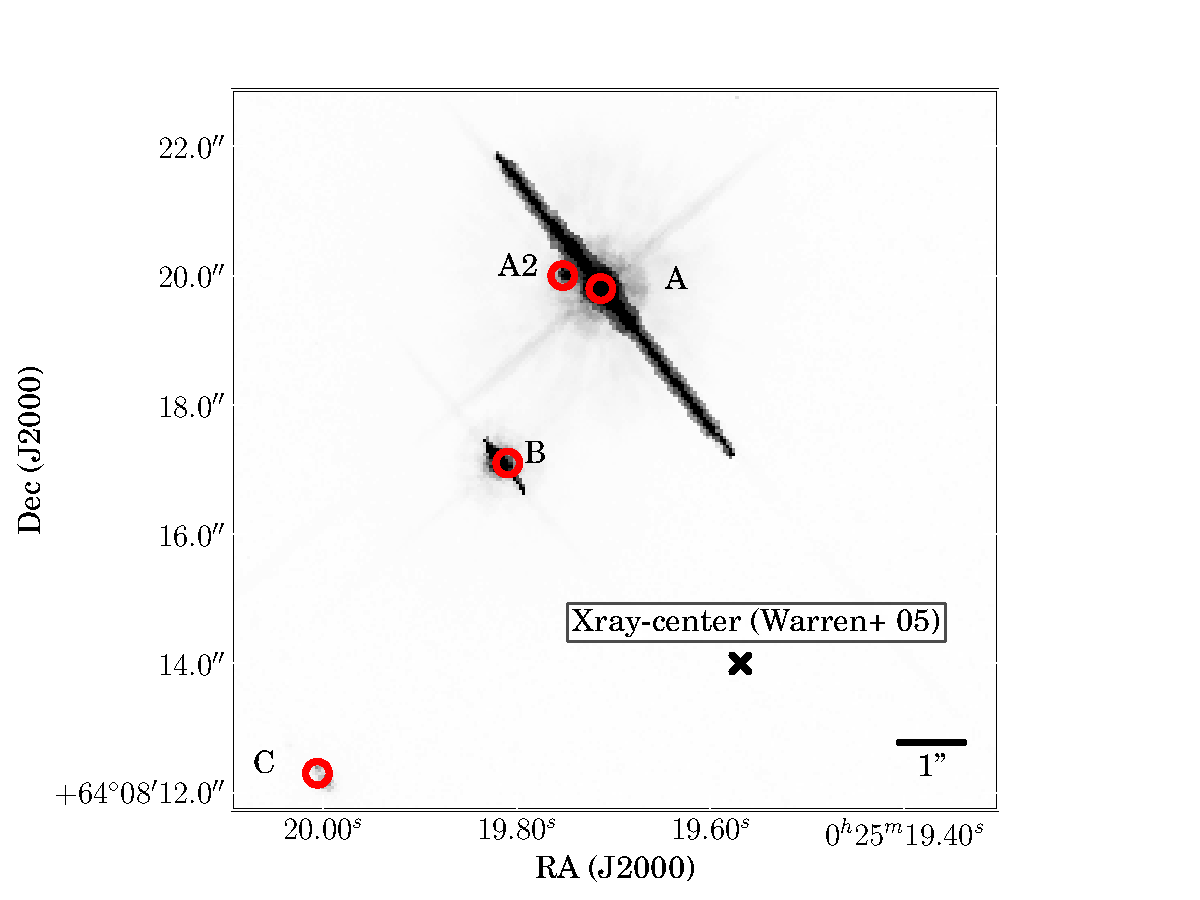
\includegraphics[width=0.7\textwidth]{chapter_conclusion/plots/overview_sn1572_a2.pdf} 
   \caption{Overview of inner region of the remnant of SN1572. All labelled stars except Star-A2 have existing high-resolution spectra. Tycho-A2 is located very close to Tycho-A (0.6\arcsec). Spectroscopy can only be obtained with adaptive optics in the infrared.}
   \label{fig:stara2_overview}
\end{figure}

The bottom line for both SN1572 and SN1006 seems to be: No bright progenitors. There are as always caveats, but we do think that with current theoretical knowledge and current instrumentation it is not worthwhile to scrutinize these remnants further. The only exception is to undertake photometrically deep observations of these remnants and look for a hot white dwarf. 

\section{The curious case of Kepler}

The last of the young remnants and the most distant one \citep[][estimates a distance of $\ge 6$\,\kpc]{2008ApJ...689..231V}.  The morphology of this remnant is not as clean and spherical as for SN1006 and SN1572 (see Figure \ref{fig:sn1604_observations}). For a long time SN1604 (Kepler's supernova) was also believed to be a \snib, but prominent iron emission in \xray spectra \citep{2007ApJ...668L.135R} suggests this event to be a \snia \citep{1995ApJ...444L..81H}. SN1604 also shows an abundance in nitrogen which is unusual for a \snia. \citet{1991ApJ...366..484B} and \citet{2003A&A...407..249S} suggest that the remnant itself posseses a very high systemic velocity of  $\approx 250\,\kms$. A recent study by \citet{2011arXiv1103.5487C} suggests that a \sd-scenario with an AGB star as a donor would explain all the observed peculiarities. They make the prediction that this star should be visible and very bright post-explosion. 

\begin{figure}[htbp] %  figure placement: here, top, bottom, or page
   \centering
   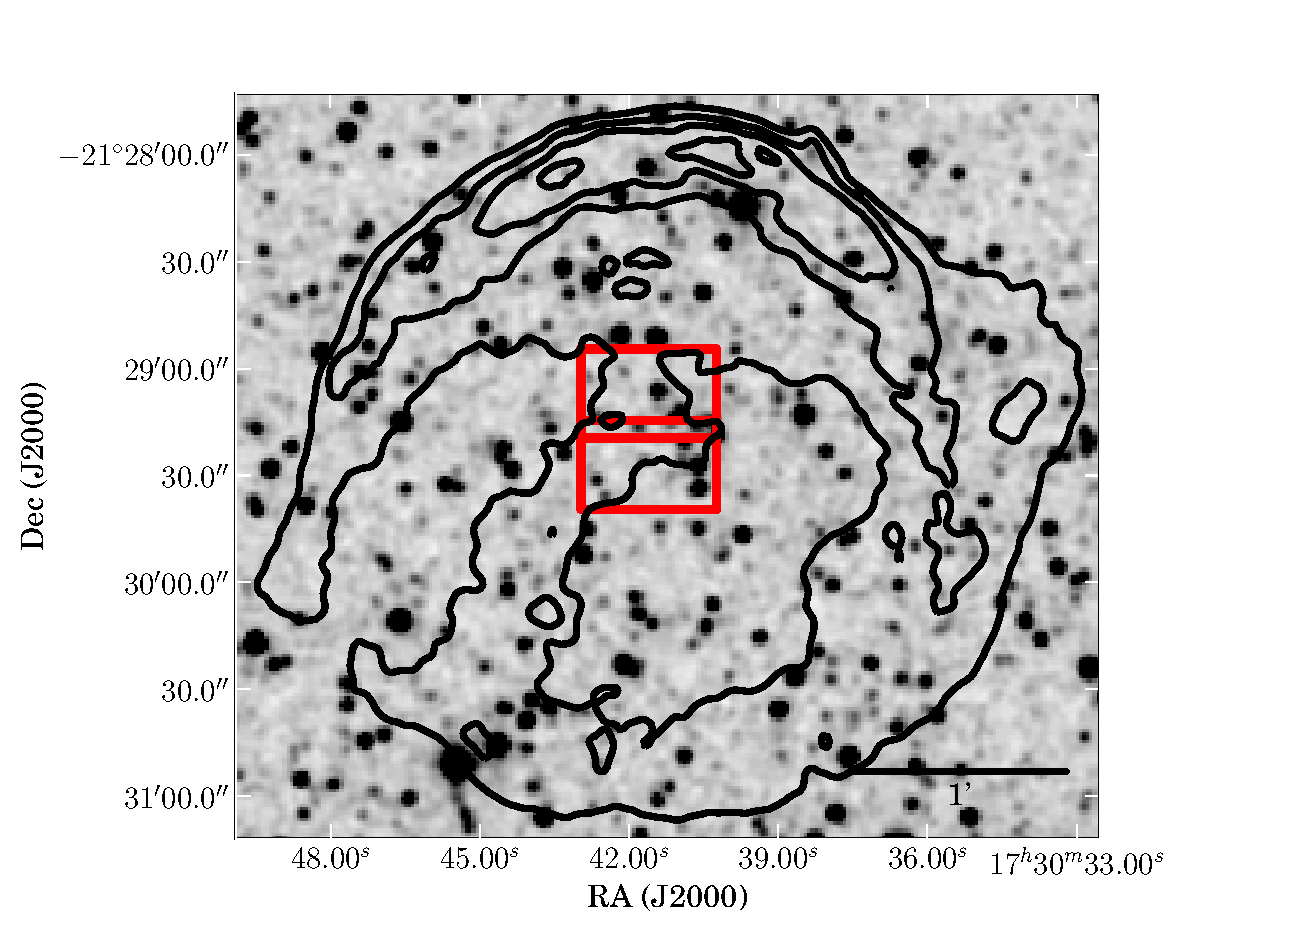
\includegraphics[width=0.7\textwidth]{chapter_conclusion/plots/sn1604_overlay.pdf} 
   \caption{VLA contours of Kepler's remnant (SN1604) overlayed on a \twomass\ image. The red rectangle show the overlapping north and south field of our WiFeS observing campaign.}
   \label{fig:example}
\end{figure}

We have obtained data with the WiFeS integral field spectrograph. The field of view for this instrument. is rectangular with dimensions of $25\arcsec \times 38\arcsec$. We have two overlapping fields that cover all stars at a projected velocity of 1300\,\kms (assuming a distance of 6\,\kpc). Extracting stellar spectra from our poor seeing data ($> 1.5\arcsec$) is technically challenging and we have not invested much time in this project.

\section{Divide et impera}

Maybe finding the progenitors of \sneia\ is too difficult using our current techniques. It might be much easier to employ the successful ``Divide et Impera'' - ``Divide and Conquer'' strategy. By asking many very small questions it might be easier to uncover on the truth than to try to solve this problem at once. We believe that one of these important questions is the mass at which \gls{cowd} explode. There are currently two main scenarios. The favored scenario is the explosion of the \gls{cowd} close to \gls{mchan} (1.38\,\msun). As shown in Chapter \ref{chap:intro} the burning of a 1.38\,\msun \gls{cowd} only produces the right abundance pattern when introducing a delayed detonation. When exploding a 1\,\msun \gls{cowd} this problem does not exist, a detonation of such a star produces the right optical photosheric spectrum. The main problem with these sub-Chandrasekhar mass explosions is that there exists no caveat free theory for the ignition yet. One key to find the explosion mass of any given \snia\ might be the abundance of stable in nebular spectra. In the Chandrasekhar mass case there should be more stable iron, in the case of a sub-Chandrasekhar mass there should be less.

\section{Dalek}

The title of this thesis suggests that \snia-progenitors and their explosions are mutually exclusive fields of research. In the previous section we have however shown that the mass of the white dwarf does have an influence on the yield. This mass is again linked to different progenitor channels. The analysis of spectra might not only help us constrain the elemental yields and explosion energies, but also give us insight into the progenitors. 

In Chapter \ref{chap:dalek} we describe a project to automate the analysis of \snia-spectra. The currently manual operated \gls{mlc}-code is ideal for automating as it strikes the right balance between speed and realism. We researched several numerical optimization strategies for this project before settling on \glspl{ga}. For now we have successfully fitted only one supernova spectrum. We are currently fine-tuning the algorithm and have enlisted the help of experts in the \gls{ga}-field. 

\section{Trouble in Paradise}

During the work of this thesis the field of \snia-research has changed significantly. When we started the donor star search there seemed little doubt in the community about the \sd-scenario. Over the recent years the \sd-channel has been seriously shaken and there has been some newfound support for the \dd-channel. The renaissance of the \dd-scenario, however often comes from the face that the merging of two white dwarfs doesn't provide as strong predictions as the \sd-scenario. This contention has reinvigorated the field of \snia progenitors and makes it a challenging and intriguing area to work in.

New transient and all sky surveys will soon start drowning us in a deluge of data. Currently the astronomical community is ill equipped to deal with such large amounts of data. This is not suprising as most astronomers are experts in physics and not data processing. This problem is not unique to astronomy, more and more fields are gathering much more data than is ever processable by individuals. We believe this is a great opportunity to start cross-disciplinary research. The fundamentals of science (e.g. pattern recognition) are definitley not unique to individual areas. New areas of science like eScience are trying to provide techniques and tools for scientists irregardless of the field. 

We have tried to conduct cross-disciplinary research in automatically fitting \sneia-spectra. Stephan Hachinger (the expert in manual fitting) and me initially have tried using the methods that were tought to us during our undergraduate years in physics (e.g. Newton-Raphson). These methods are still useful for very simple problems, however do not scale to today's highly non-linear problems with many co-dependant variables. Sam Inverso, a computer scientist working many in the area of neuro-science, joined us first and helped us do our first baby-steps in \glspl{ga}. His help has advanced the \gls{dalek} to its present state. In the last half year two new members have joined the team, whose research is in numerical optimization. They are very interested in applying their techniques to ``real world'' problems, which are scarce in the optimization community.

This work definitley tries to show: Multidisciplinary research is not only a buzzword, but can advance individual fields of science much faster than they could advance in isolation.


